\chapter{Getting Acclimated}

\justify
Let's start by considering the objectives for this book:
\justify
\begin{itemize}
\item
  Create an extensible lab environment for rapid prototyping and
  development. Get out of our old comfort zone, into a new one.
\item
  Keep our lab costs down while meeting the rest of the objectives.
  Utilize free services and open source tools to the extent possible.
\item
  Use the published best practices for each tool we choose to employ.
\item
  Always leave our project in a functional state.
\end{itemize}

\justify
The ideas captured here are not means to any end. Rather, these are meant to be starting points, giving you a frame of reference with novel technologies and techniques that will streamline your projects. You will build up the momentum to pursue these new ideas by following along with the examples outlined in this book.

\justify
You should work to build up a solid base of code examples and problem solving techniques that will greatly increase your efficacy. Over time, new tools and processes will rotate in and out of your toolbox as technology progresses. Keep in mind that your job is to maintain that momentum, to keep experimenting and to see what is useful enough to stick with you and make a permanent part of your repertoire.

\justify
Companies often make their services free in the hopes that you will see the value and usefulness of their products. The thinking goes that hopefully you will see enough utility that you will recommend them to your enterprise clients and integrate their products into your workflows. Not a bad trade-off! It only makes sense to avail yourself o free-tier cloud services, build and test platforms, and low or no-cost hosting environments. There are plenty of these out there and we will explore some of these as we dive further into the topics.

\justify
When we choose to use a tool, say Ansible for example, it only makes sense to also adopt the most up-to-date and best practices for using that tool. File system layout, naming conventions, script syntax and organization, and so on. We get to enjoy the clear and safe path forged by the folks that came before us, and with whom we share many goals.

\justify
Finally, the authors have found it very helpful for their peace of mind
to leave projects clean and green, to the extent possible, before walking away from the keyboard for the day. Perhaps you would find similar benefit should you choose to adopt this practice.

\section{Prerequisites}

\justify
This book intends to be a practical treatment of common and popular
technologies from the DevSecOps world. As such, we assume the reader has
some basic knowledge of certain concepts. We will be exploring new ways
of working for folks who are somewhat familiar with:

\begin{itemize}
\item
  Linux (UI and command line)
\item Python 3
\item
  Familiarity with github.com and the concepts of {pull requests} and \href{}{branching}.
\end{itemize}

\justify
The examples in this book have been tested on Linux running the latest
version of Docker.

\justify
Let's take a look at some of the other foundational environmental
elements we need in place to be successful.

\subsubsection{Windows Specific Prerequisites}

\begin{itemize}
\item installation of power shell
\item installation of python 3.9.x
\item installation of gh or github command line client
\end{itemize}

\subsubsection{Linux Specific Prerequisites}
\justify
When installing Docker on Linux hosts, it should be noted that docker-compose must be installed separately.

\section{The Workhorse (IDE)}
\justify
It is quite helpful to have a piece of software on your workstation that
makes code creation and edits easier. This software is commonly known as
an Integrated Development Environment (IDE)\index{Integrated Development Environment (IDE)}.

\justify
One of the key features to look for in an IDE is to use one that you
don't have to spend a lot of time configuring and maintaining. A decent
IDE with the right add-ons can provide syntax highlighting to show
potential issues you might have missed, help you check for spelling or
grammar mistakes in your documentation, and even makes suggestions on
alternate ways of writing your code.

\justify
Visual Studio Code\footnote{\url{https://code.visualstudio.com/Download}}
from Microsoft is quite a popular choice these days in a large sea of
commercial and Open Source candidates. VSCode\index{VSCode} works well on Linux, Mac
and other operating systems. The environment is easily extensible to
support most any language, linter, or syntax checker we may have a need
for, thanks to their easy to use and well integrated "Extensions"
feature. VSCode also has an integrated terminal window\index{Terminal Window} so the developer
can execute shell commands without leaving the IDE screen.
 
\justify
Folks also seem to be quite fond of the Sublime\footnote{\url{https://www.sublimetext.com/}} IDE for similar reasons, including it's customizability and extensibility.

single: Sublime

\begin{figure}
\centering
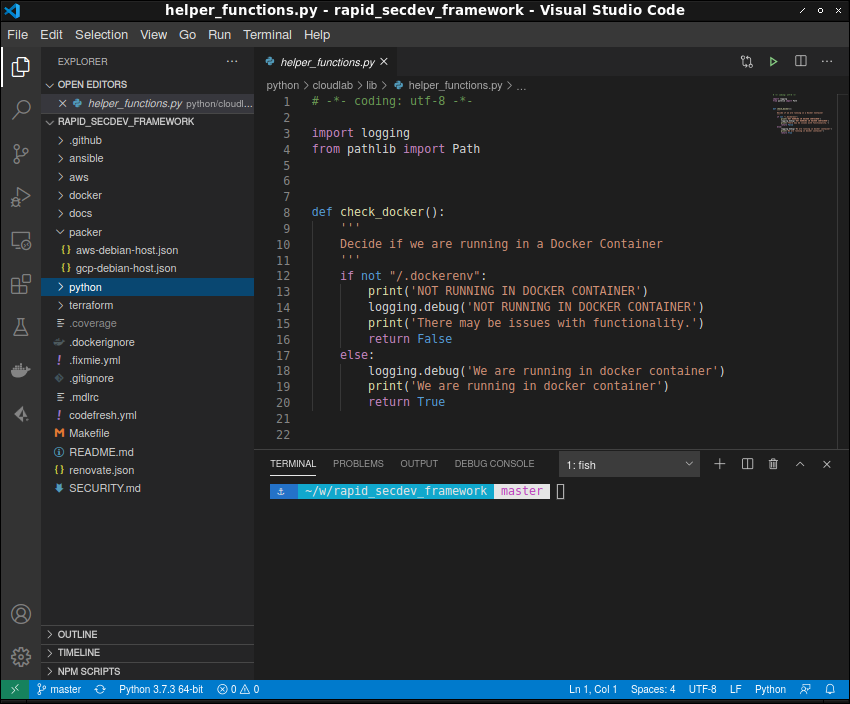
\includegraphics[scale=0.45]{../images/setup-vscode.png}
\caption{The VScode IDE.}
\end{figure}

\section{The Flow (Pipelines)}

\justify
Work products such as code and documents begin their life on developer workstations. We will refer to these developer environments where this takes place as the "local" environment. These work products are created, reviewed and checked into Revision Control Systems (RCS), GitHub for example, by the DevSecOps practitioner. Other revison control systems include GitLab and BitBucket.

single: Revsion Control System (RCS)

\justify
Test cases are created and run against the work products at check-in time, to ensure stability, security, and compatibility with the existing code base. The automation required to execute tests every time work is checked in is also typically the responsibility of the DevSecOps engineers. As seen in {myFig1} work typically "flows" from the local environments, into a test environment, and finally to production where
it is available for use by the entire user base.

\justify
We will refer to the entirety of this three-stage flow as one example of
a "pipeline". Code from one or more local environments is checked in to
the revision control system throughout a typical DevSecOps workday, and
continuously tested and integrated with the main code base. That is to
say, work undergoes "Continuous Integration" (CI) with the main code base, and often "Continuous Delivery" (CD) between local, test, and production environments. This is where the term "CI/CD Pipeline" comes from.

single: pipeline single: CI single: Continuous Deployment single: CD
single: Continuous Integration

\begin{figure}
\centering
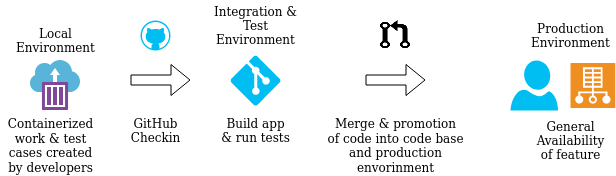
\includegraphics[scale=0.63]{../images/flow.png}
\caption{Typical build pipeline.}
\end{figure}

\justify
While the CI/CD Pipeline is often the primary focus of the DevSecOps
engineer, other pipelines exist as well. For example, let's assume our
organization maintains a vast pool of raw data, also known as a data
lake. The staff Data Engineers build and maintain Data Science pipelines
to facilitate the smooth flow of logs and other data into that data
lake. Now Data Scientists are able to create machine learning models
that rely on that data to produce useful insights. As another example,
consider code changes as they move from developer workstations into a
code repository for storage. Accessing this code for the purpose of
testing will differ from how it is accessed for the purposes of
deployment. The order of operations and flow between differing
functions might be said to comprise two different pipelines.

single: Data Lake single: Data Science

\subsection{Shifting Left}
\justify
We now have a mental picture of how software will flow from Development,
to Test, and to Production.

single: Shift Left

\subsection{Automation}
\justify
Consider what may happen when we want to apply the lessons from this book across a large environment made up of many hosts, containers, pieces of application software, etc. It becomes a huge challenge to log in to each host or container individually. Typing, or even cutting and pasting commands to keep things up and running properly, look at logs,
and so on becomes problematic.

\justify
This is where automation comes in. Automation is a way to provision and maintain some or many hosts in a programmatic and touchless manner. Automation is the force multiplier we use to achieve scaling.

single: Automation single: scaling

\subsection{Agile Methodologies}

\justify
The concept of Agile Software development is an expansive topic unto itself. Although we won't implicitly dedicate a lot of our time to these ideas, agile is widely regarded as an underpinning of a successful
DevSecOps program.

single: Agile

\subsection{Lab Exercises}
\justify
This book is meant to be a workbook as much as it is meant to be read. You are encouraged to jump ahead, go back and re-read, do the exercises you think you can apply the learning objective from right away, and skip the parts you don't think you will ever use. Learning can be a non-linear experience and you are encouraged to "color outside the lines" to the extent you feel comfortable doing so.

\justify
That said, I've attempted to give this book a feel of moving the reader along towards a final project. This project is meant to guide the reader through applying the information introduced between this chapter and that.
